\chapter{Aplicación de Deep Leaning en SHM con sensores de deformación}%ANN}

%  -----------------------------------------  %


\section{Proyecto INESASSE}

El Proyecto INESASSE (Integración y Explotación de Sistemas de Autodiagnóstico y Supervisión de Salud Estructural en aviones no tripulados) tiene como objetivo principal investigar la capacidad de implantación, en condiciones operativas, de sistemas de supervisión estructural (SSE), empleando redes de sensores de fibra óptica.

Este proyecto de investigación fue realizado por el INTA (Instituto Nacional de Técnica Aeronáutica), en conjunto con la ETSIAE (Escuela Técnica Superior de Ingeniería Aeronáutica y del Espacio), y consta de 3 fases:

\begin{enumerate}
    \item Elaboración de un modelo de elementos finitos (FEM) del sistema estructural, a través del cual se establece la morfología de la red de sensores. Sobre este FEM se simularán distintos daños producidos sobre la estructura, a fin de analizarlos mediante distintas técnicas SHM y determinar la posición óptima de la red sensorial.
    \item Fabricación de dos estructuras idénticas de CFRP que se instrumentaran con la red de sensores definida en la fase 1, integrables en el UAV en cuestión. Tras esto, a una de estas estructuras se le realizará una campaña de ensayos en tierra a fin de validar los FEM, además de comparar los resultados obtenidos mediante herramientas SHM sobre el modelo teórico y el real. Al igual que en el FEM, se realizarán los mismos daños estructurales controlados.
    \item  En la última fase del proyecto, la estructura fabricada anteriormente que no fue ensayada, se integrará en un UAV en operaciones de vuelo reales, procesando datos de los sensores integrados en la fase 2, e investigando las capacidades del sistema SHM seleccionado para el vuelo.
\end{enumerate}

El vehículo aéreo no tripulado que protagoniza este proyecto es el UAV Milano, con una masa en servicio de 900 kg y una autonomía de hasta 20 horas. En la Figura \ref{mialno} se puede apreciar una imagen del mismo.

\begin{figure}[ht]
    \centering
    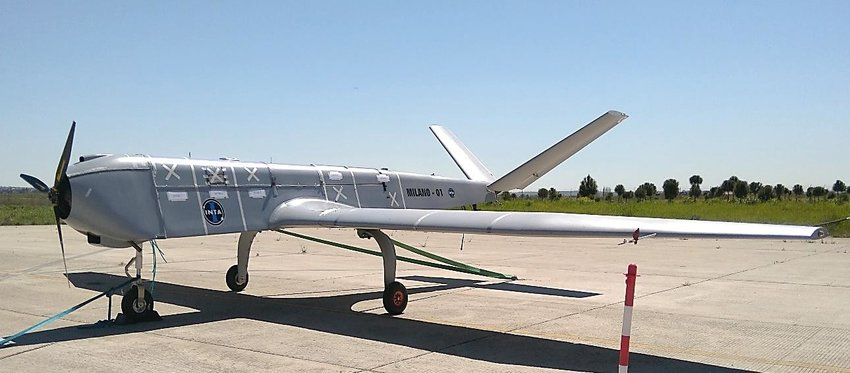
\includegraphics[width=120mm]{3/Fotos/Milano.png}
    \captionsetup{justification=centering,margin=1.25cm}
    \caption{UAV INTA Milano}
    \label{mialno}
\end{figure}


%----------%


\subsection{Estructura y red de sensores}

La estructura de la aeronave sobre la que se ha realizado el FEM y se ha fabricado después es el fuselaje posterior del UAV Milano. Esta estructura está compuesta por:

\begin{itemize}
    \item[\tiny$\bullet$] Revestimiento inferior con un larguero longitudinal en T dividido en dos y refuerzos sobre las pestañas. Fabricado con cinta UD fuera de autoclave.
    \item[\tiny$\bullet$] Revestimiento superior con dos largueros en L y refuerzos sobre las pestañas. Fabricado con cinta UD fuera de autoclave.
    \item[\tiny$\bullet$] Cuatro cuadernas con refuerzos sobre las mismas. Fabricadas con cinta UD fuera de autoclave.
    \item[\tiny$\bullet$] Dimensiones aproximadas de $2600 x 850 x 890$ mm.
\end{itemize}

En la Figura \ref{estructura_fuselaje} se puede ver el diseño explosionado de los componentes descritos.

\begin{figure}[ht!]
    \centering
    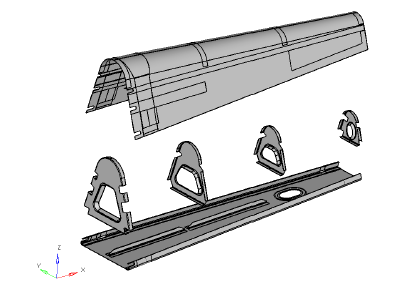
\includegraphics[width=130mm]{3/Fotos/estructura_fuselaje.png}
    \captionsetup{justification=centering,margin=1.25cm}
    \caption{Fuselaje posterior}
    \label{estructura_fuselaje}
\end{figure}

Sobre esta estructura se van a distribuir dos redes de sensores de fibra óptica, uno formado por sensores FBG y otro por OBR. Con ellos se recogerá el campo de deformaciones de la estructura que se procesará para obtener la clasificación de los daños. En las Figuras \ref{FBG_sensores} y \ref{OBR_sensores} se tiene una representación gráfica de la posición de estas redes en la estructura.

\begin{figure}[ht]
    \centering
    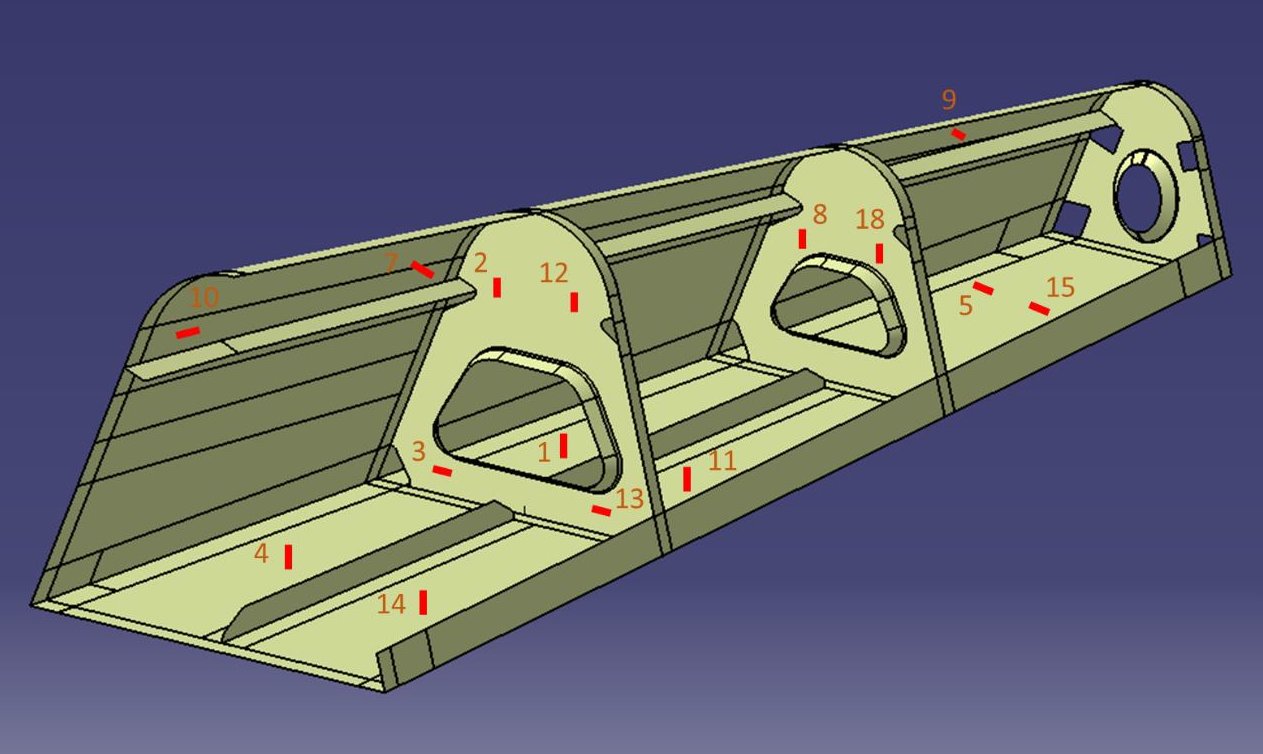
\includegraphics[width=125mm]{3/Fotos/FBG.png}
    \captionsetup{justification=centering,margin=1.25cm}
    \caption{Red de sensores FBG}
    \label{FBG_sensores}
\end{figure}

\begin{figure}[ht!]
    \centering
    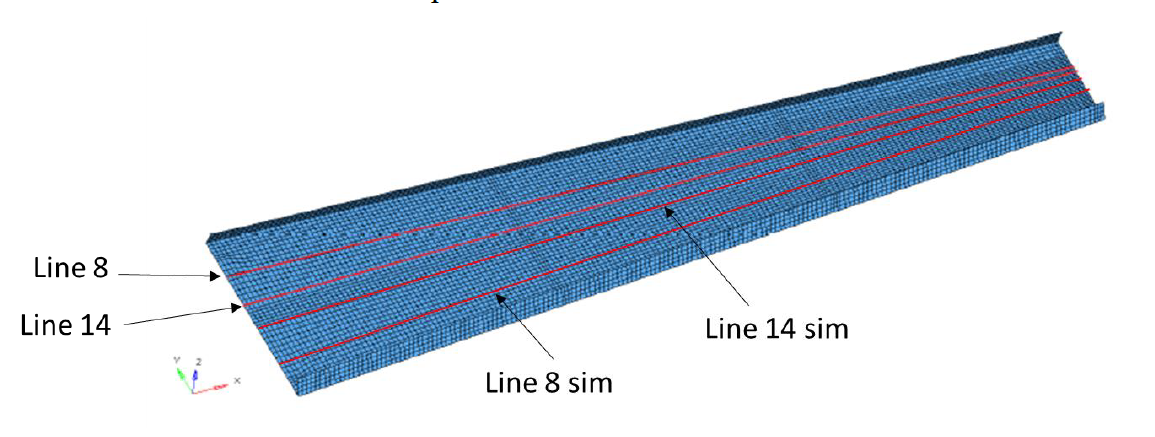
\includegraphics[width=130mm]{3/Fotos/OBR_1.png}
    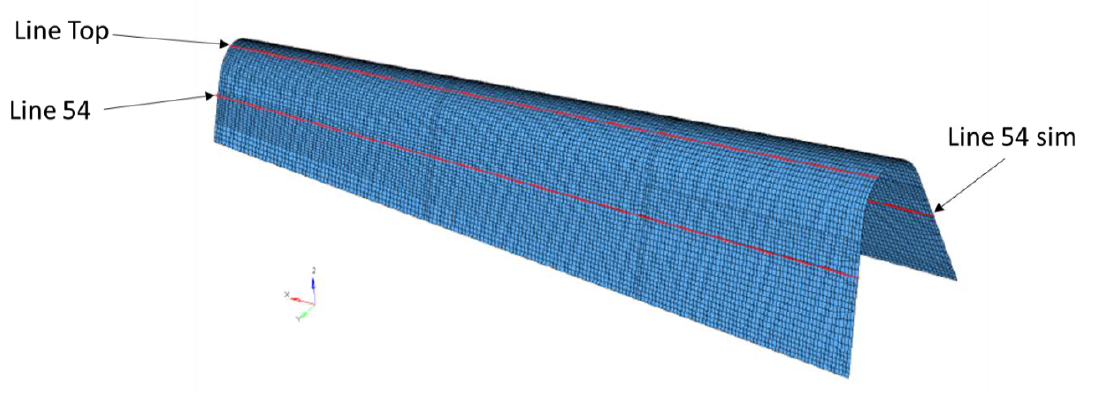
\includegraphics[width=130mm]{3/Fotos/OBR_2.png}
    \caption{Red de sensores OBR}
    \label{OBR_sensores}
\end{figure}

Es importante indicar que, puesto que los sensores de medida distribuida son unidireccionales, se han obtenido las deformaciones en la dirección longitudinal de la fibra (tracción/compresión).

%----------%

\subsection{Planteamiento de daños y descripción de ensayos} 

El objetivo de este proyecto es tener un sistema SHM para detectar daños en un fuselaje de material compuesto durante su operación, por lo tanto, se necesita definir la localización de estos daños y sus tamaños.

Estos daños corresponden con desencolados parciales o totales en las zonas que se definirán a continuación. En la Figura \ref{dam} se puede ver la localización de cada daño en la estructura y en la Tabla \ref{tdam} se pueden ver sus caracterísitcas.

\begin{figure}[ht]
    \centering
    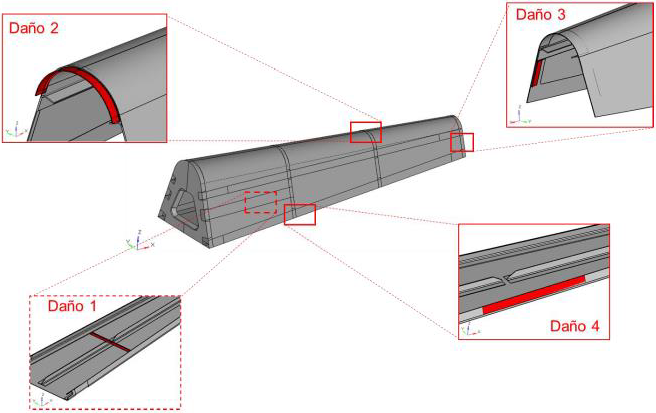
\includegraphics[width=125mm]{3/Fotos/dam.png}
    \caption{Esquema de los daños realizados a la estructura}
    \label{dam}
\end{figure}

\begin{table}[h!]
    \centering
    \begin{tabular}{ | m{12.5mm} | m{37.5mm}| m{30mm} |  m{25mm} |  m{25mm} |}  \hline
        \textbf{\footnotesize{DAÑO}}& \textbf{\footnotesize{TIPO DE DAÑO}} & \textbf{\footnotesize{ELEMENTOS AFECTADOS}} & \textbf{\footnotesize{LONGITUD MÁXIMA}} & \textbf{\footnotesize{INCREMENTO}}\\ 
        \hline
        D1 & Desencolado parcial del pie de la cuaderna & Cuaderna 2, revestimiento inferior & 450 mm & 30 mm \\ 
        \hline
        D2 & Desencolado parcial de la pestaña superior de la cuaderna & Cuaderna 3, revestimiento superior & 350 mm & 25 mm \\ 
        \hline
        D3 & Desencolado parcial de la pestaña lateral de la cuaderna & Cuaderna 4, revestimiento superior & 180 mm & 30 mm \\ 
        \hline
        D4 & Desencolado parcial entre el revestimiento inferior y el revestimiento superior & Revestimiento inferior, revestimiento superior & 900 mm & 30 mm \\ 
        \hline
    \end{tabular}
    \caption{Definición de daños en el fuselaje}
    \label{tdam}
\end{table}

Es importante resaltar que, aunque el ensayo estructural y las simulaciones se realizaron para los cuatro daños, se llegó a la conclusión de que el daño 3 era irrelevante tras ver los resultados obtenidos. Por lo tanto, dicho daño fue descartado.\\

Para facilitar el trabajo a los operarios que realizaron los ensayos del fuselaje, se sustituyó la unión adhesiva por uniones remachadas. Esto permitió controlar mejor la progresión de los daños y también que fueran reparados tal y como se ve en la Figura \ref{remaches}.

\begin{figure}[ht]
    \centering
    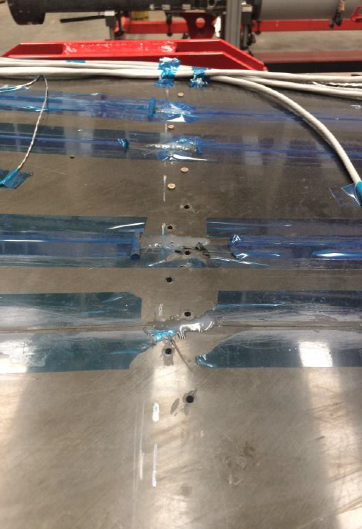
\includegraphics[width=55mm]{3/Fotos/remaches.png}
    \captionsetup{justification=centering,margin=1.25cm}
    \caption{Realización del daño por extracción de remaches}
    \label{remaches}
\end{figure}

Los ensayos sobre la estructura real se simularon también siguiendo la misma configuración en el FEM. Las condiciones de contorno a las que está sometido el fuselaje son las siguientes:

\begin{itemize}
    \item[\tiny$\bullet$] Empotramiento en la sección de unión con el fuselaje anterior
    \item[\tiny$\bullet$] Carga vertical en la sección de unión con la cola
\end{itemize}

El ensayo comienza con la estructura descargada y se aplica la carga de forma escalonada. La carga va aumentando 400 N en 10 escalones hasta llegar a un máximo de 4 kN.

La configuración del banco de ensayos se puede ver en la Figura \ref{ensayo}

\begin{figure}[ht]
    \centering
    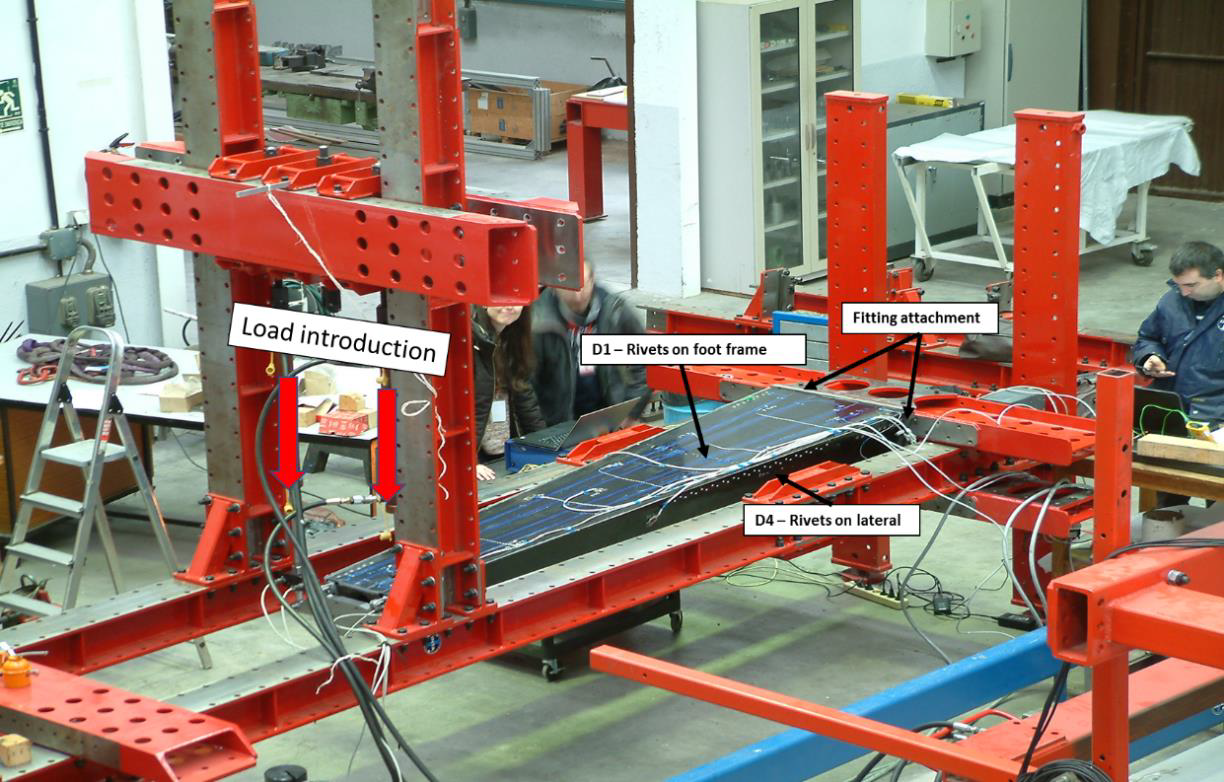
\includegraphics[width=145mm]{3/Fotos/ensayo.png}
    \captionsetup{justification=centering,margin=1.25cm}
    \caption{Vista general de la configuración de los ensayos}
    \label{ensayo}
\end{figure}


%----------%


\subsection{Modelo de elementos finitos}

Se va a hacer un breve resumen de las características del FEM utilizado. Este modelo consta de 62802 grados de libertad, el tamaño medio de sus elementos es de 15 mm, y está formado por:
\begin{itemize}
    \item[\tiny$\bullet$] 26181 nodos
    \item[\tiny$\bullet$] 34080 elementos quad4 (Ratio máximo de 4.768)
    \item[\tiny$\bullet$] 25 elementos tria3 (Ratio máximo de 6.219)
\end{itemize}

Los elementos tria3 del modelo se encuentran principalmente en las cuatro cuadernas debido a que su geometría es más complicada de mallar que la del resto del fuselaje.\\

En la Figura \ref{femest} se pueden ver los distintos elementos del modelo y en cuales de ellos se introducen las condiciones de contorno.

\begin{figure}[h!]
    \centering
    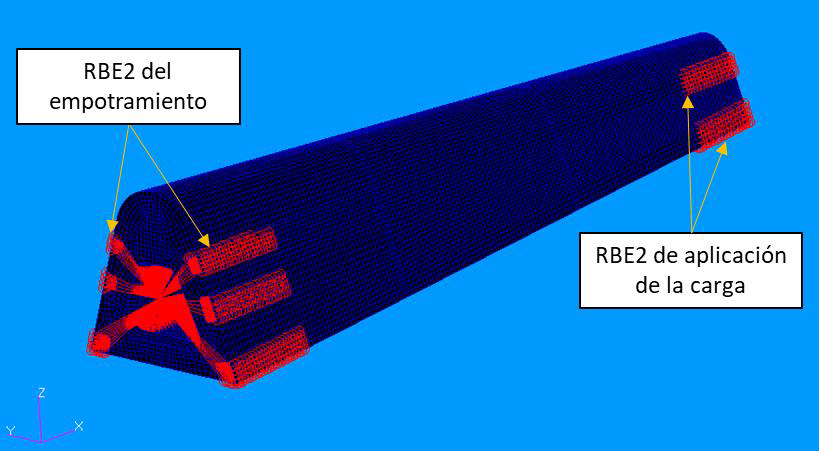
\includegraphics[width=120mm]{3/Fotos/femest.png}
    \captionsetup{justification=centering,margin=1.25cm}
    \caption{Modelo de elementos finitos del fuselaje posterior del UAV Milano}
    \label{femest}
\end{figure}


%----------%

\clearpage

\section{Pre-procesado de señales}

Una vez que se han realizado los ensayos y simulaciones, es necesario pre-procesar los datos recogidos por las redes de sensores para ajustarlos en contenido y forma para que las redes neuronales puedan realizar una clasificación correcta.

Los datos que se obtienen de los ensayos reales se van a tratar de forma diferente a los obtenidos a través del FEM, por ello, este apartado está separado en dos grupos, \textit{Ensayo real} y \textit{FEM}.

\subsection{Ensayo real}
    
La red de sensores FBG registra las deformaciones de forma ininterrumpida durante el ensayo completo, dando así una curva de deformación frente al tiempo para cada uno de los sensores distribuidos en la estructura, como se puede ver a continuación en la Figura \ref{def_t}.\\
    
\begin{figure}[h!]
    \centering
    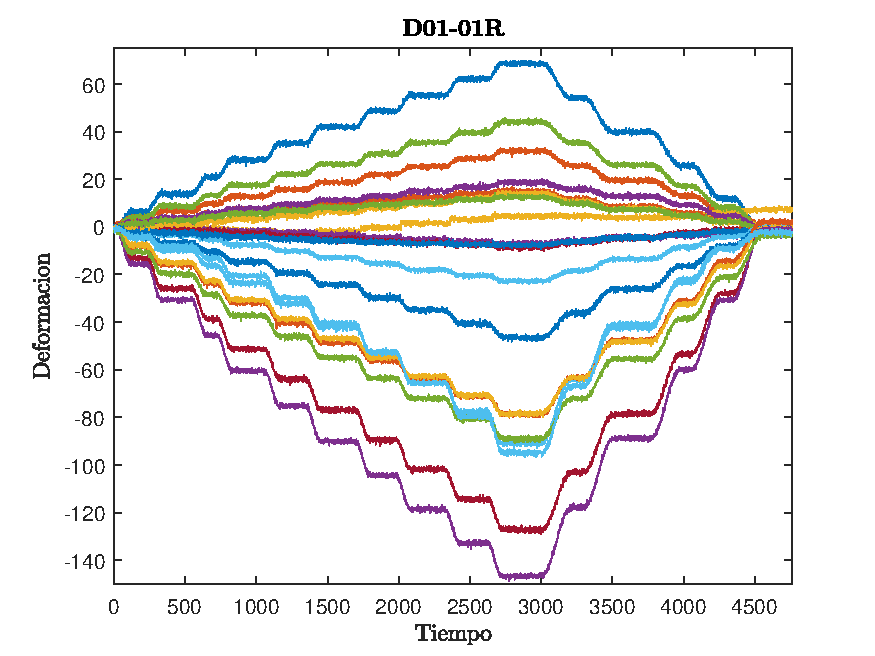
\includegraphics[width=125mm, angle=0]{3/Fotos/Sensores_FBG.pdf}
    \captionsetup{justification=centering,margin=1.25cm}
    \caption{Medida de todos los sensores durante el ensayo del Daño 1 con un remache extraído}
    \label{def_t}
\end{figure}
    
Cuando los actuadores llegan a un nivel de carga paran durante un tiempo antes de aumentar o disminuir la carga aplicada con el fin de estabilizar la carga. Por lo tanto, para separar las medidas en diferentes niveles de carga hay que detectar cuando el actuador comienza a moverse. La detección de el comienzo de aplicación de carga está representada en las Figuras \ref{def_s} y \ref{def_p}.
    
\begin{figure}[h!]
    \centering
    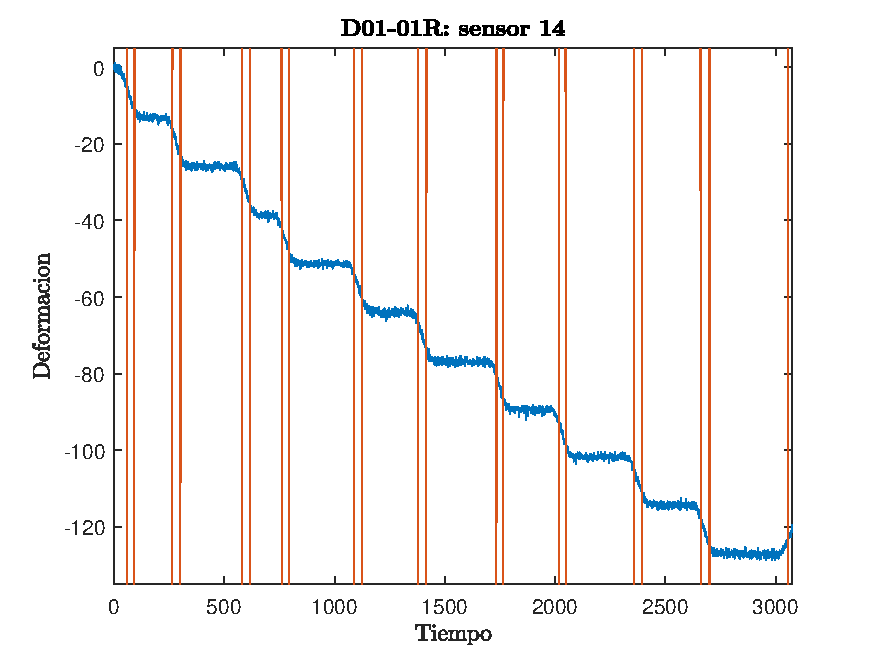
\includegraphics[width=125mm, angle=0]{3/Fotos/Saltos_FBG.pdf}
    \captionsetup{justification=centering,margin=1.25cm}
    \caption{Detección de los escalones producidos por las carga vertical}
    \label{def_s}
\end{figure}
    
\begin{figure}[h!]
    \centering
    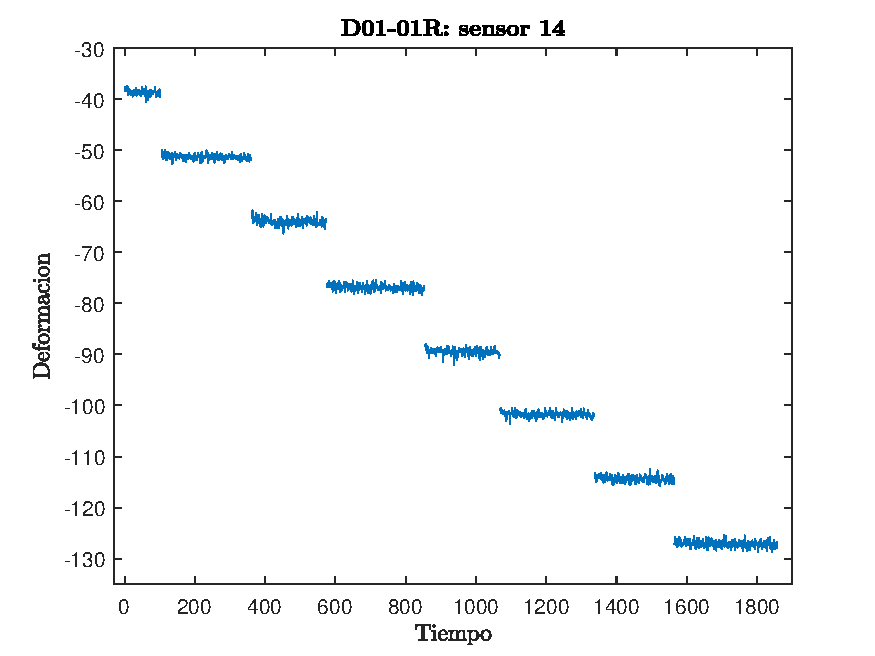
\includegraphics[width=125mm, angle=0]{3/Fotos/Procesado_FBG.pdf}
    \captionsetup{justification=centering,margin=1.25cm}
    \caption{Medidas de los sensores FBG en el ensayo preprocesadas}
    \label{def_p}
\end{figure}    
    
Finalmente se eliminan las medidas obtenidas durante la transición entre escalones usando como referencia las líneas naranjas de la Figura \ref{def_s} y se fija la carga mínima que se va a usar durante el estudio en un 30\% de la carga máxima.\\
 %Tras este proceso se obtienen múltiples ensayos individuales para cada carga y tipo de daño tal y como se ve en la Figura \ref{def_p}.
    
Una vez que se han aislado los escalones se dibuja un histograma para ver la variabilidad de los datos obtenidos. Como se ve en la Figura \ref{def_h}, los valores de las medidas se asemejan a una distribución normal con mida -127.75 deformaciones. Esto quiere decir que el ruido introducido por los sensores FBG hace que cada medida que se realiza en un tiempo diferente pueda ser considerada como un ensayo independiente. De un único ciclo de carga se obtienen una gran cantidad de datos para entrenar a la red.\\

\begin{figure}[h!]
    \centering
    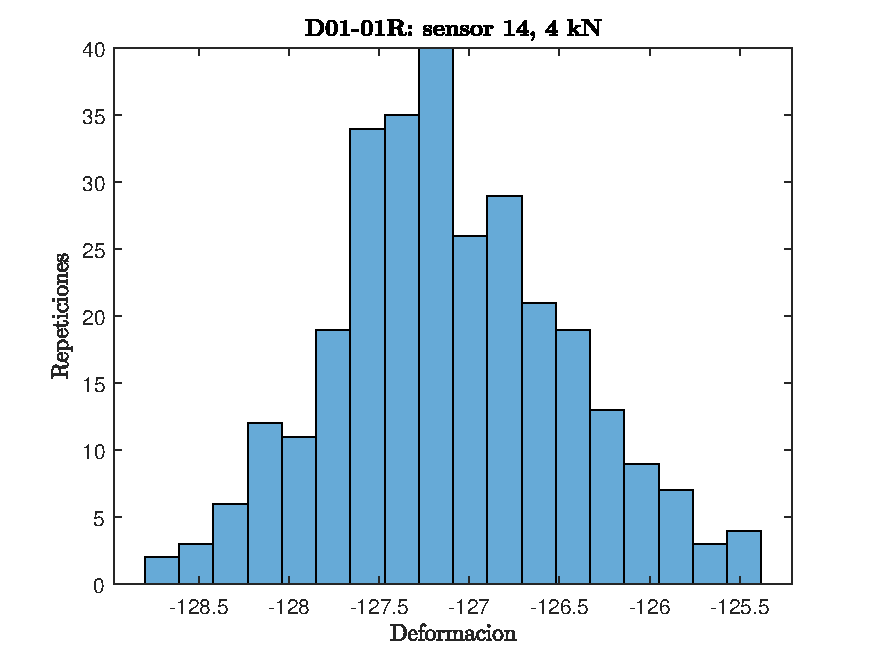
\includegraphics[width=125mm, angle=0]{3/Fotos/Histograma_FBG.pdf}
    \captionsetup{justification=centering,margin=1.25cm}
    \caption{Histograma del escalón 4 kN, 100\% de carga}
    \label{def_h}
\end{figure}    

Tras pre-procesar las señales se puede visualizar el campo de deformaciones medido por los sensores FBG para cada estado de daño y el estado sin daño o de referencia en la Figura \ref{FBGR_dam}. Al estar cada daño localizado en una zona diferente de la estructura, los cambios en el campo de deformaciones son locales y en la Figura \ref{FBGR_dif} se aprecia que sensores están más cerca de la zona dañada ya que sufren una mayor variación respecto a las medidas obtenidas de la estructura sin daño.

\begin{figure}[h!]
    \centering
    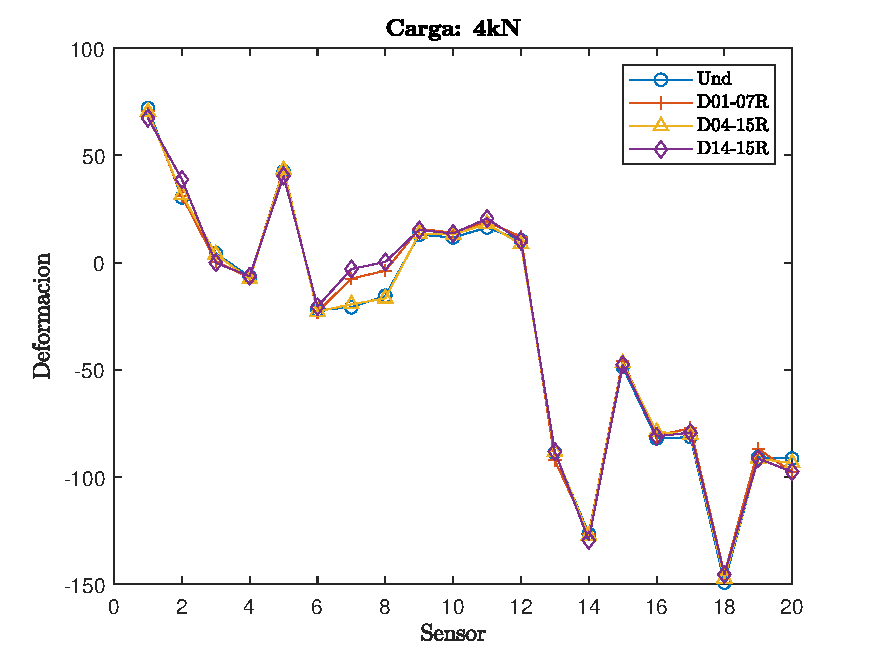
\includegraphics[width=125mm, angle=0]{3/Fotos/FBG_damages.pdf}
    \captionsetup{justification=centering,margin=1.25cm}
    \caption{Campo de deformaciones medido por los sensores FBG para todos los daños}
    \label{FBGR_dam}
\end{figure}
        
\begin{figure}[h!]
    \centering
    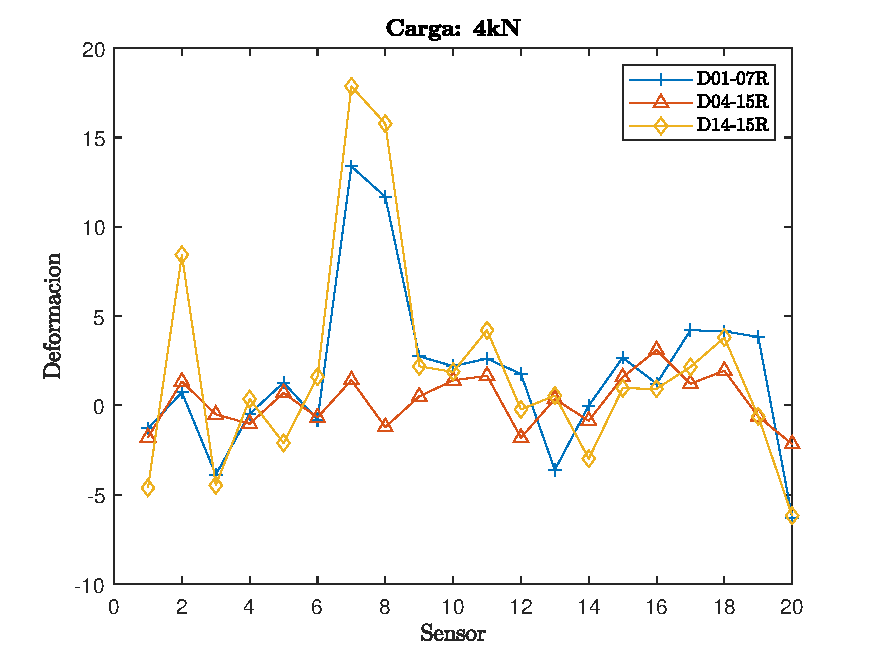
\includegraphics[width=125mm, angle=0]{3/Fotos/FBG_dif.pdf}
    \captionsetup{justification=centering,margin=1.25cm}
    \caption{Diferencia de los campos de deformaciones referenciado con el estado sin daño (FBG)}
    \label{FBGR_dif}
\end{figure}


%----------------------%

    

\vspace*{10pt}
    
Por otro lado, los sensores OBR realizan una captura instantánea del campo de deformaciones. Esto quiere decir que se tiene una única muestra para cada tipo de daño y nivel de carga (ejemplo en la Figura \ref{fig:D01-R3}), lo cual es insuficiente para conseguir unos buenos resultados con la red.\\

\begin{figure}[h!]
    \centering
    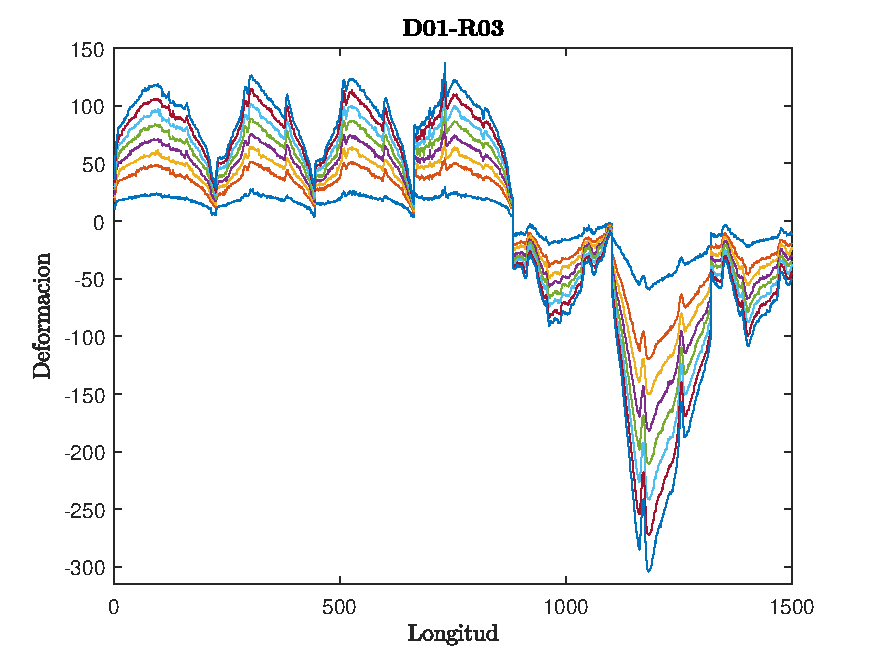
\includegraphics[width=125mm, angle=0]{3/Fotos/D01-R3.pdf}
    \captionsetup{justification=centering,margin=1.25cm}
    \caption{Campo de deformaciones provocado por el daño 1 con 3 remaches extraídos para todos los casos de carga}
    \label{fig:D01-R3}
\end{figure}
    
Siguiendo el mismo razonamiento usado con los sensores FBGs, si se añade una distribución de ruido gausiano a un valor del campo de deformaciones, se pueden generar ensayos independientes con los que entrenar a la red. Sin embargo, el campo de deformaciones de la Figura \ref{fig:D01-R3} ya contiene ruido asociado a la medida. 

Para conseguir un campo de deformaciones que usar como referencia, al que añadir posteriormente ruido, se va a utilizar el filtro \textit{Savitzky-Golay}. Este filtro digital es comúnmente usado para suavizar series de datos equiespaciados \cite{Savitzky-Golay}.

\begin{figure}[h!]
    \centering
    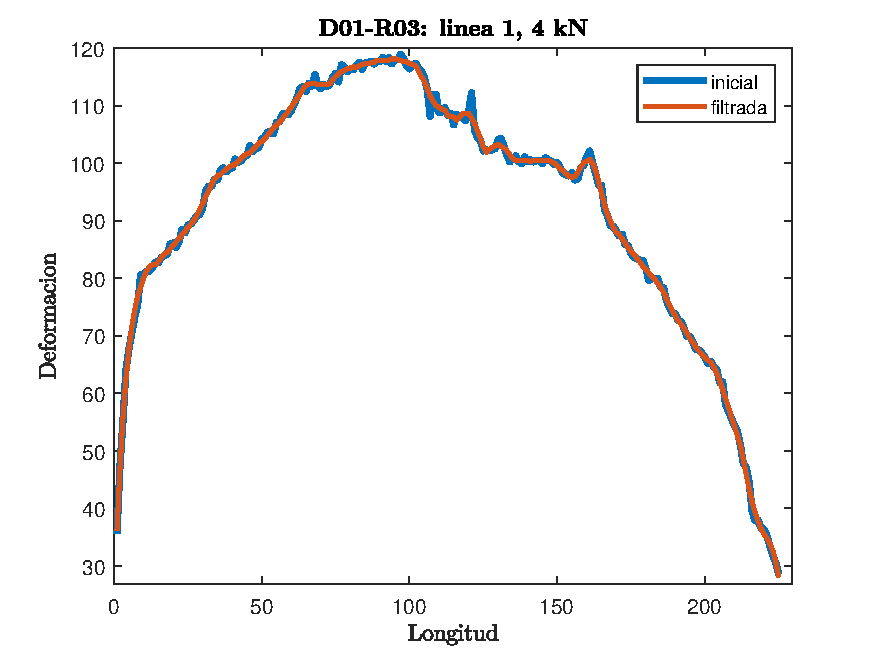
\includegraphics[width=125mm, angle=0]{3/Fotos/filtro.pdf}
    \captionsetup{justification=centering,margin=1.25cm}
    \caption{Aplicación del filtro Savitzky-Golay a una linea de sensor OBR}
    \label{fig:filtro}
\end{figure}

La diferencia entre la medida sin filtrar y filtrada se aprecia claramente en la Figura \ref{fig:filtro}.\\

Ahora que se tiene una medida de referencia, ya se puede añadir la distribución de ruido de amplitud 1.5 deformaciones (Figura \ref{OBRR_ruido}) y generar más muestras.
    
\begin{figure}[h!]
    \centering
    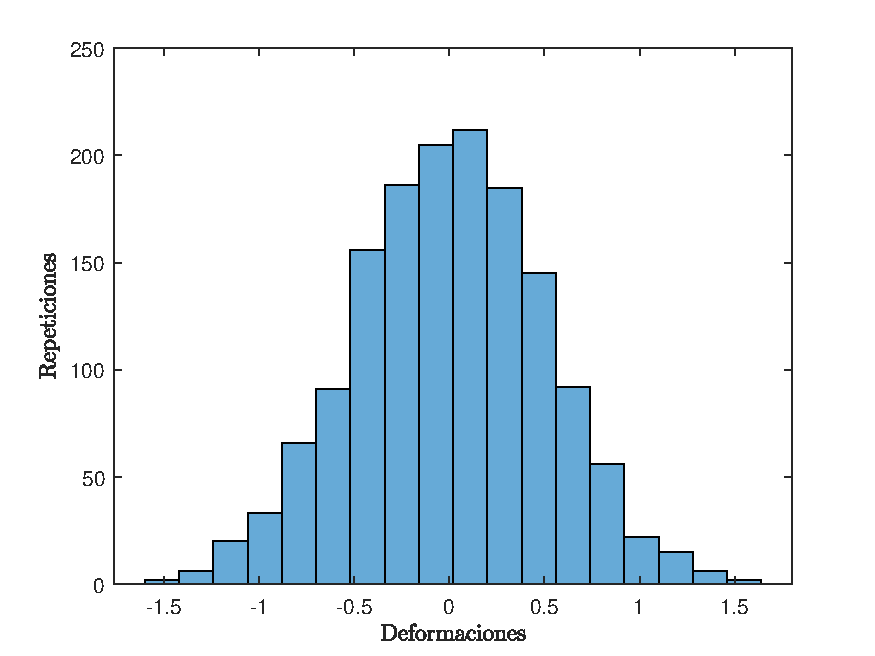
\includegraphics[width=125mm, angle=0]{3/Fotos/histo_ruido_OBR.pdf}
    \captionsetup{justification=centering,margin=1.25cm}
    \caption{Distribución de ruido gausiano con amplitud 1.5 deformaciones}
    \label{OBRR_ruido}
\end{figure}
    
En la Figura \ref{fig:OBRR_det} se puede ver un detalle del caso D01-R03 en el que se ha ampliado las deformaciones medidas por una línea de sensor. Aquí se aprecia más claramente que cada una de estas muestras se pueda considerar como un ensayo independiente.
    
\begin{figure}[h!]
    \centering
    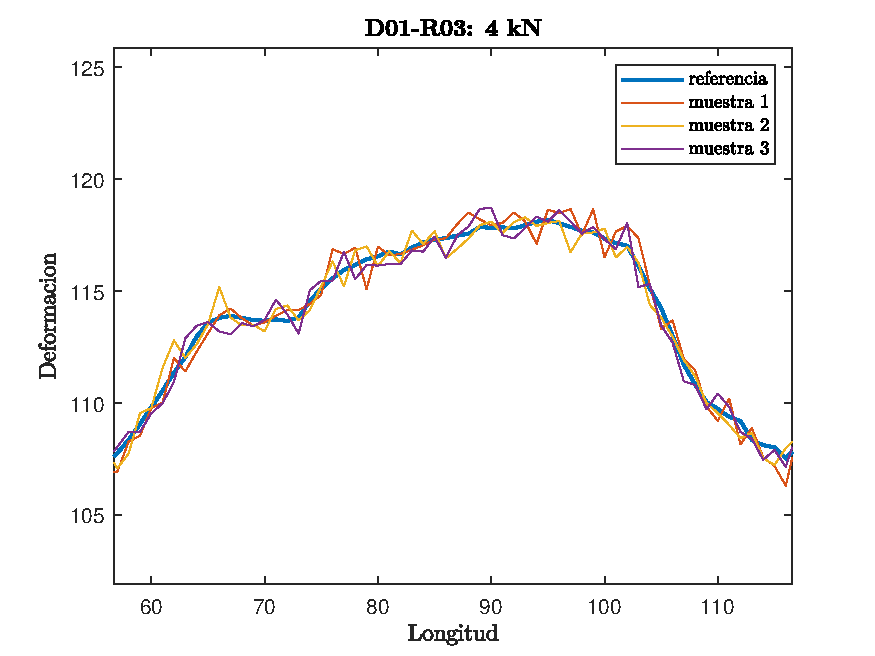
\includegraphics[width=125mm, angle=0]{3/Fotos/detalle_OBR_ruido.pdf}
    \captionsetup{justification=centering,margin=1.25cm}
    \caption{Detalle de las variaciones provocadas por el ruido gausiano}
    \label{fig:OBRR_det}
\end{figure}
   
Igual que se ha hecho con los FBGs, en las Figuras \ref{OBRR_dam} y \ref{OBRR_dif} se pueden ver los campos de deformaciones provocados por los distintos daños con la carga máxima y su diferencia respecto al estado sin daño.

\begin{figure}[h!]
    \centering
    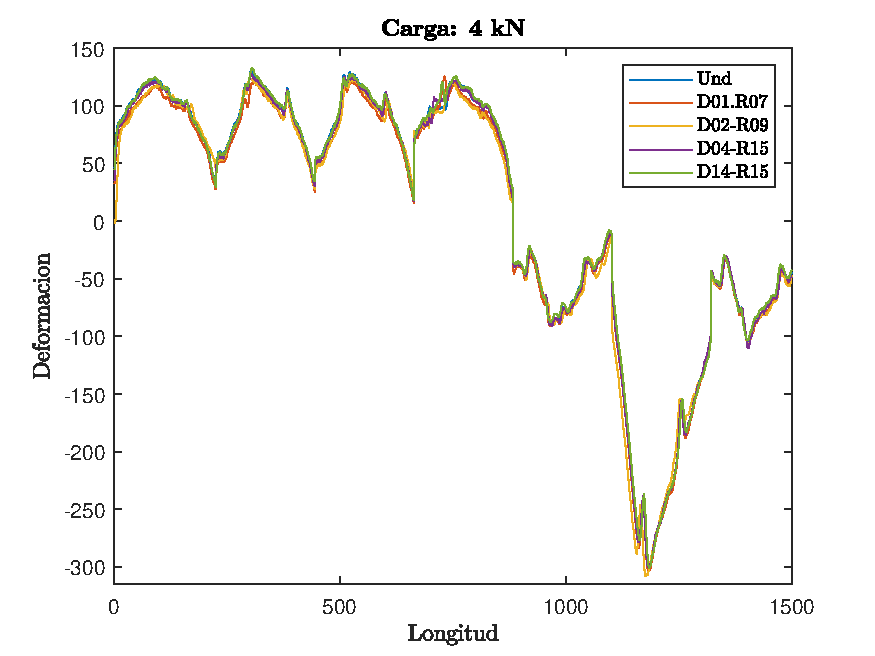
\includegraphics[width=125mm, angle=0]{3/Fotos/OBR_damages.pdf}
    \captionsetup{justification=centering,margin=1.25cm}
    \caption{Campo de deformaciones medido por el sensor OBR para todos los daños}
    \label{OBRR_dam}
\end{figure}
    
\begin{figure}[h!]
    \centering
    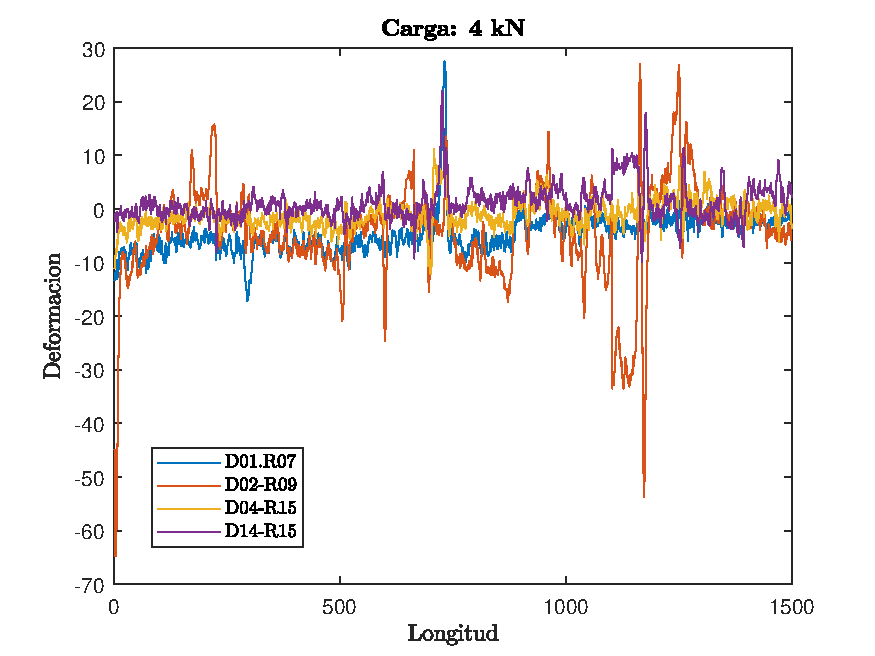
\includegraphics[width=125mm, angle=0]{3/Fotos/OBR_dif.pdf}
    \captionsetup{justification=centering,margin=1.25cm}
    \caption{Diferencia de los campos de deformaciones referenciado con el estado sin daño (OBR)}
    \label{OBRR_dif}
\end{figure}
    
    
%----------%
    
\subsection{FEM}
    
% A diferencia del ensayo de la estructura real, las simulaciones solo se han realizado introduciendo la carga máxima puesto que se supone que que el material no supera el límite elástico y, por lo tanto el campo de deformaciones de la estructura es proporcional a la carga aplicada. 
    
% Para obtener los niveles de carga como en el ensayo lo que se ha hecho es multiplicar las deformaciones por un factor de carga con un mínimo de 30\% y espaciados en intervalos de 10\% (8 en total).\\
    

\url{https://towardsdatascience.com/hands-on-graph-neural-networks-with-pytorch-pytorch-geometric-359487e221a8}


%  -----------------------------------------  %

\clearpage

\section{Construcción del modelo de Deep Learning}

Una vez que se han procesado las deformaciones se tiene un \textit{Dataset} para los sensores FBG en el que cada muestra es de dimensión 20 (20 sensores) mientras que en el dataset de los sensores OBR las muestras son de dimensión 1499 (equivalente a tener 1499 sensores).

Un ser humano no puede visualizar un espacio con tantas dimensiones. Esto hace complicado tener una idea de la distribución de las muestras y mucho menos imaginar como la red genera fronteras entre las distintas clases de datos( como se ha explicado en \hyperref[sec:funcionamiento_DL]{\textit{Representación gráfica del funcionamiento una NN}}).\\

Para reducir la dimensionalidad de los datasets y tener una representación gráfica de ellos se va a utilizar un algoritmo de Machine Learning muy popular para la visualización de datos multidimansionales: \textbf{t-SNE (t-distributed Stochastic Neighbor Embedding)}. A continuación se va a hacer una rápida explicación del funcionamiento de este algoritmo \cite{t_sne}.\\

\textit{Stochastic Neighbor Embedding (SNE)} comienza convirtiendo las distancias euclideas entre puntos del dataset de alta dimensionalidad en probabilidades condicionales que representan su similitud. La similitud del punto $x_j$ con el punto $x_i$ es la probabilidad condicional $p_{j|i}$ y su proximidad se calcula usando una distribución de densidad de probabilidad gaussiana centrada en $x_i$. Para los puntos cercanos, el $p_{j|i}$ es relativamente alto, mientras que para los puntos lejanos, el $p_{j|i}$ será casi infinitesimal. Matemáticamente, el la probabilidad condicional $p_{j|i}$ viene dada por la Ecuación \ref{eq:prob_alta}.

\begin{equation}
	p_{j|i} = \frac{exp(-||x_i-x_j||^2/2\sigma ^2_i)}{\sum_{k\neq i}( exp(-||x_i-x_k||^2/2\sigma ^2_i)}
	\label{eq:prob_alta}
\end{equation}
\vspace{4pt}

En el espacio de baja dimensión los puntos $y_i$ y $y_j$ son la transformación de $x_i$ y $x_j$ del espacio con alta dimensionalidad. Es posible calcular una probabilidad condicional similar, $q_{j|i}$ a la anterior. Para ello, fijamos la varianza del gaussiano que se emplea en el cálculo de las probabilidades condicionales $q_{j|i}$ en $\frac{1}{\sqrt{2}}$. Por lo tanto, modelamos la similitud del punto $y_j$ con $y_i$ con la Ecuación \ref{eq:prob_baja}

\begin{equation}
	q_{j|i} = \frac{exp(-||y_i-y_j||^2)}{\sum_{k\neq i}(exp(-||y_i-y_k||^2)}
	\label{eq:prob_baja}
\end{equation}
\vspace{4pt}

Si los puntos $y_i$ y $y_j$ del mapa de baja dimensionalidad modelan bien la similaridad entre los puntos $x_i$ y $y_j$ del espacio con alta dimensionalidad, las probabilidades $p_{j|i}$ y $q_{j|i}$ serán iguales. Por lo tanto, el objetivo de SNE es minimizar las discordancias entre $p_{j|i}$ y $q_{j|i}$.\\

Igual que para las NN, es necesario tener una función de costes que represente el error que está cometiendo el algoritmo y así optimizarla por medio del descenso del gradiente. La función de costes elegida es la divergencia Kullback-Leibler individual entre las distribuciones de probabilidad conjunta, P y Q (Equación \ref{eq:costes}).

\begin{equation}
	C = KL(P||Q) = \sum_{i}\sum_{j}p_{ji}\log\frac{p_{j|i}}{q_{j|i}}
	\label{eq:costes}
\end{equation}
\vspace{4pt}



\section{Resultados}

\subsection{INESASSE}

\begin{itemize}
    \item[$\bullet$] \textbf{CLASIFICACIÓN DE CARGA}
    
    \begin{figure}[h!]
        \centering
        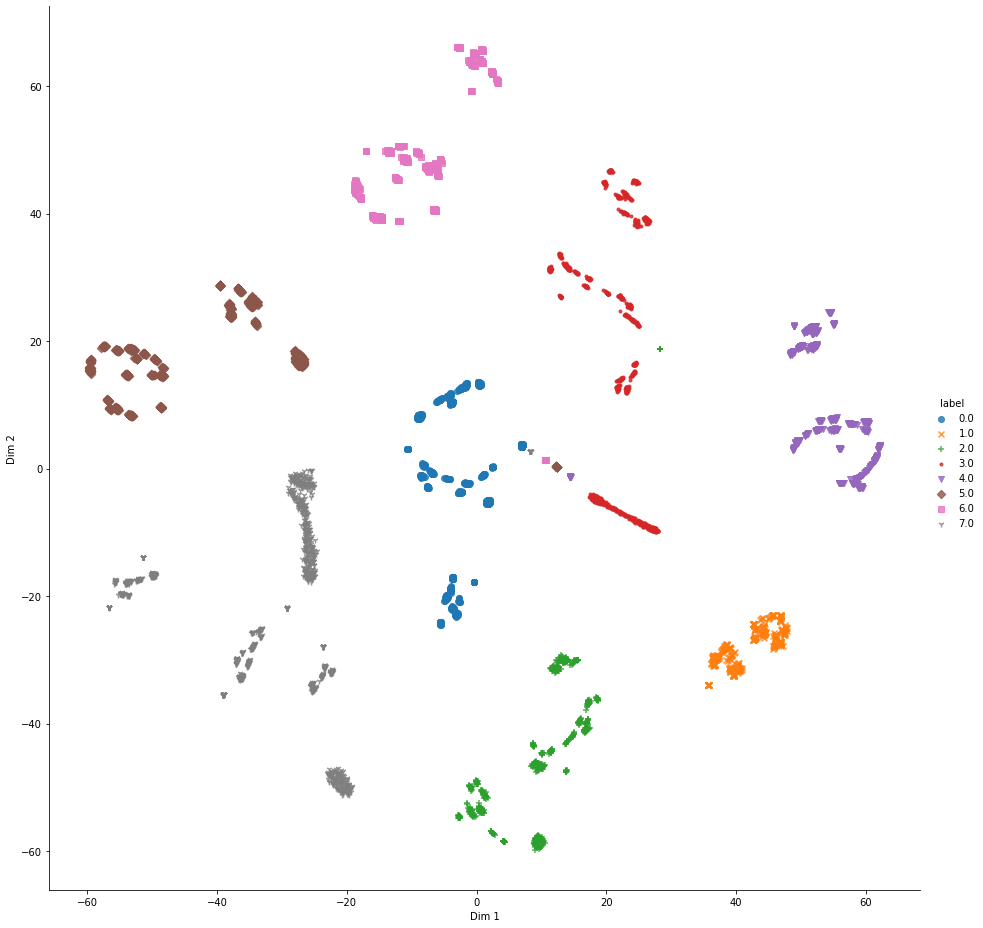
\includegraphics[width=150mm]{3/Fotos/Load_INESASSE_t-sne.png}
        \captionsetup{justification=centering,margin=1.25cm}
        \caption{Representación de los vectores de deformaciones tras reducir la dimensión de 20 a 2}
        \label{def_h}
    \end{figure}  
    
    \begin{figure}[h!]
        \centering
        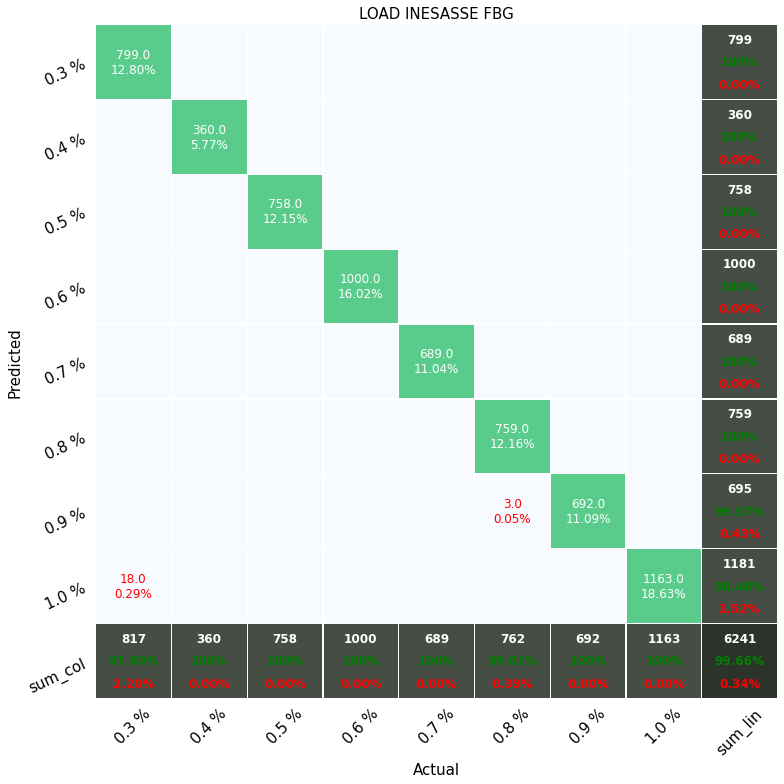
\includegraphics[width=150mm]{3/Fotos/Load_INESASSE_confusion.png}
        \captionsetup{justification=centering,margin=1.25cm}
        \caption{Matriz de confusión}
        \label{def_h}
    \end{figure}  
    
    \item[$\bullet$] \textbf{CLASIFICACIÓN DE CASO DE DAÑO}
    
    \begin{figure}[h!]
        \centering
        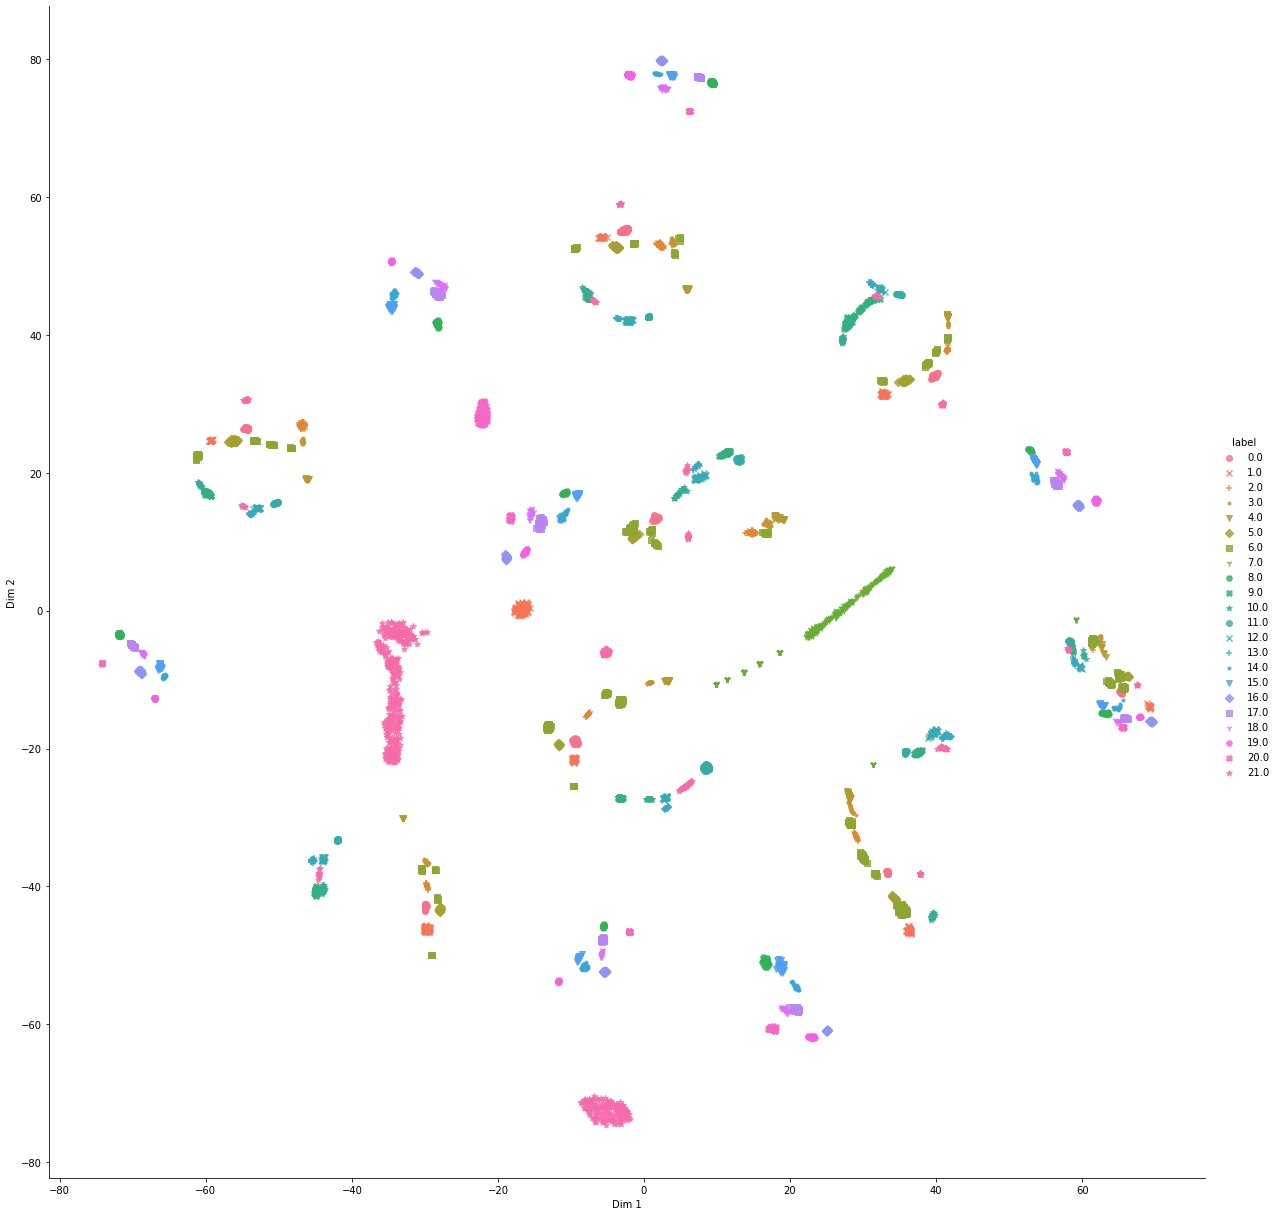
\includegraphics[width=150mm]{3/Fotos/Ty_Si_INESASSE_t-sne.png}
        \captionsetup{justification=centering,margin=1.25cm}
        \caption{Representación de los vectores de deformaciones tras reducir la dimensión de 20 a 2}
        \label{def_h}
    \end{figure}  
    
    \begin{figure}[h!]
        \centering
        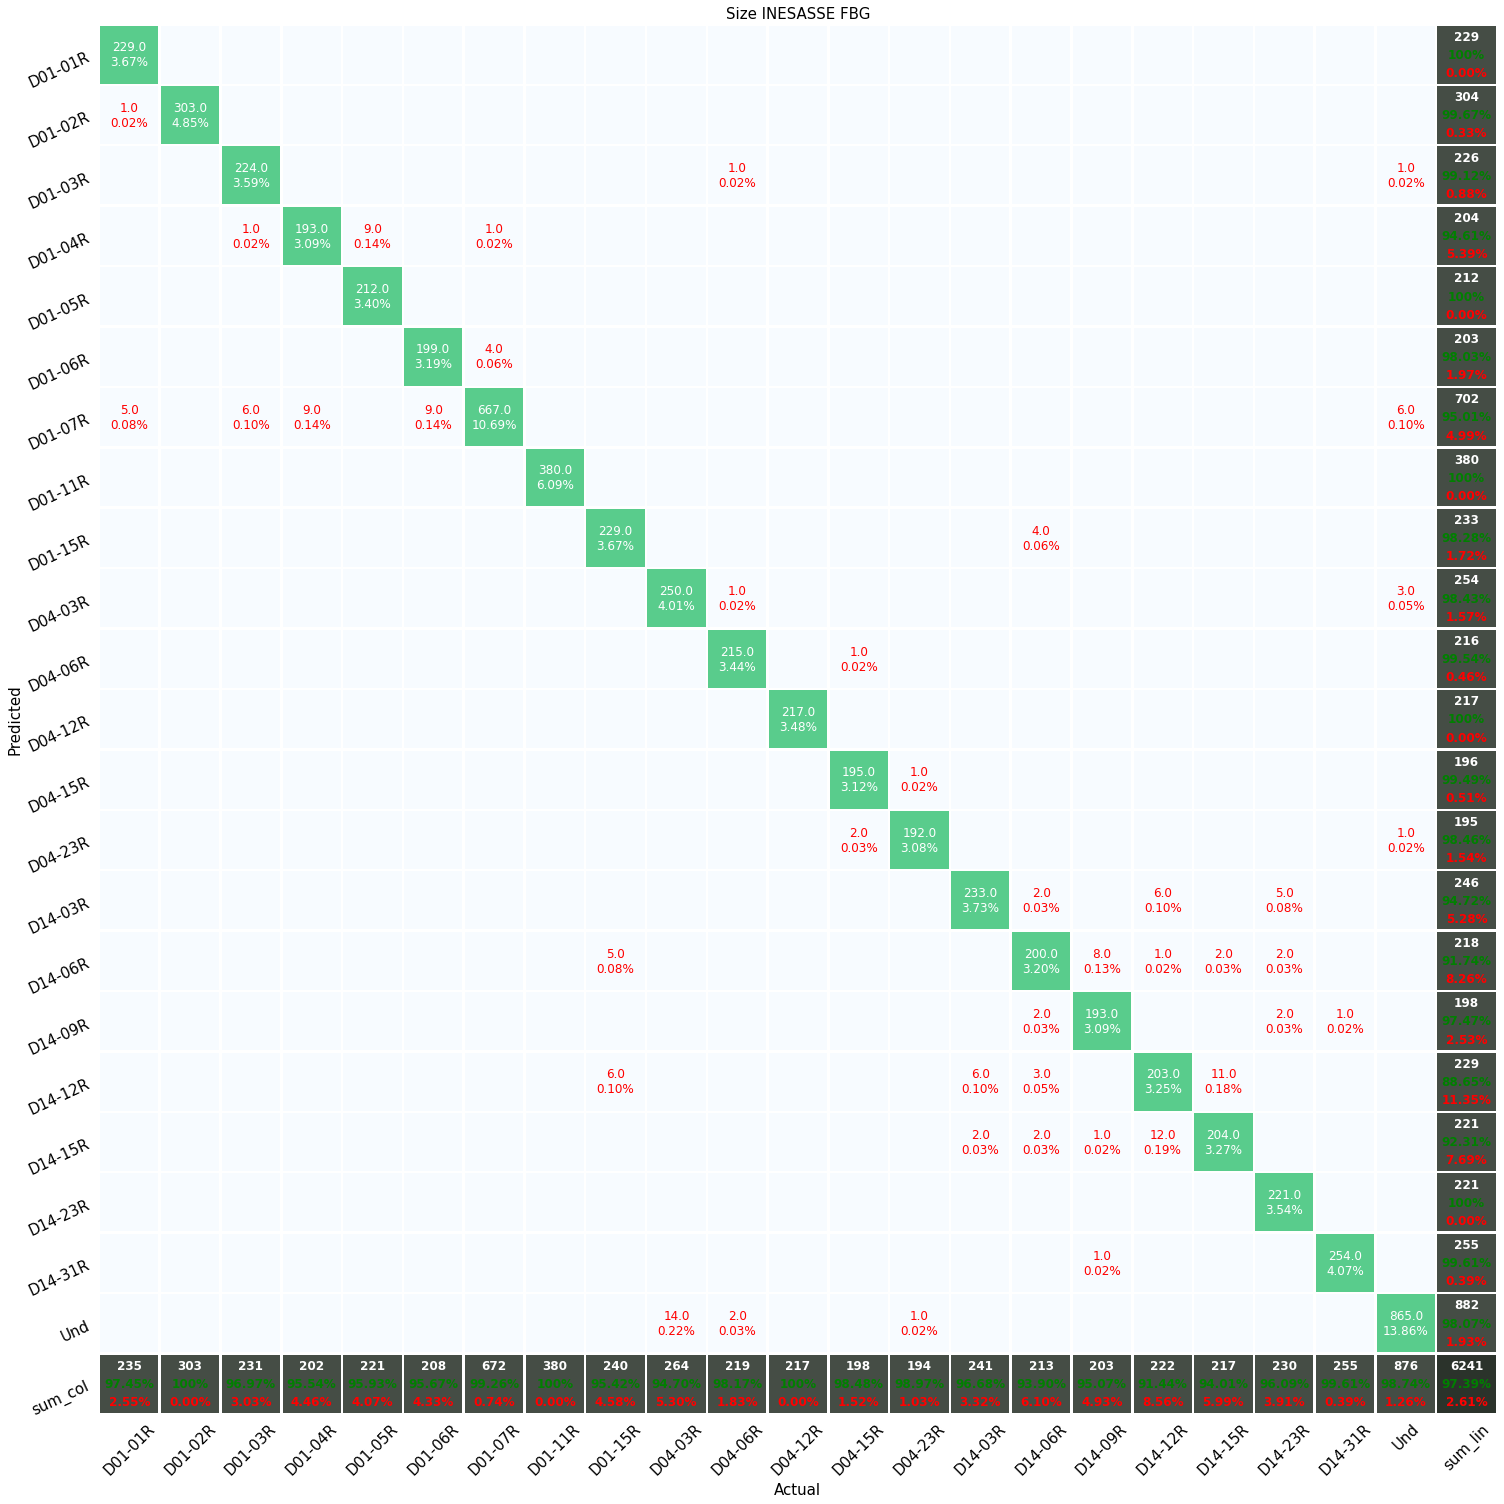
\includegraphics[width=150mm]{3/Fotos/Ty_Si_INESASSE_confusion.png}
        \captionsetup{justification=centering,margin=1.25cm}
        \caption{Matriz de confusión}
        \label{def_h}
    \end{figure} 
    
\end{itemize}


%------------------%


% \subsection{DACOMAT}

% \begin{itemize}
%     \item[$\bullet$] \textbf{CLASIFICACIÓN DE CARGA}
    
%     \begin{figure}[H]
%         \centering
%         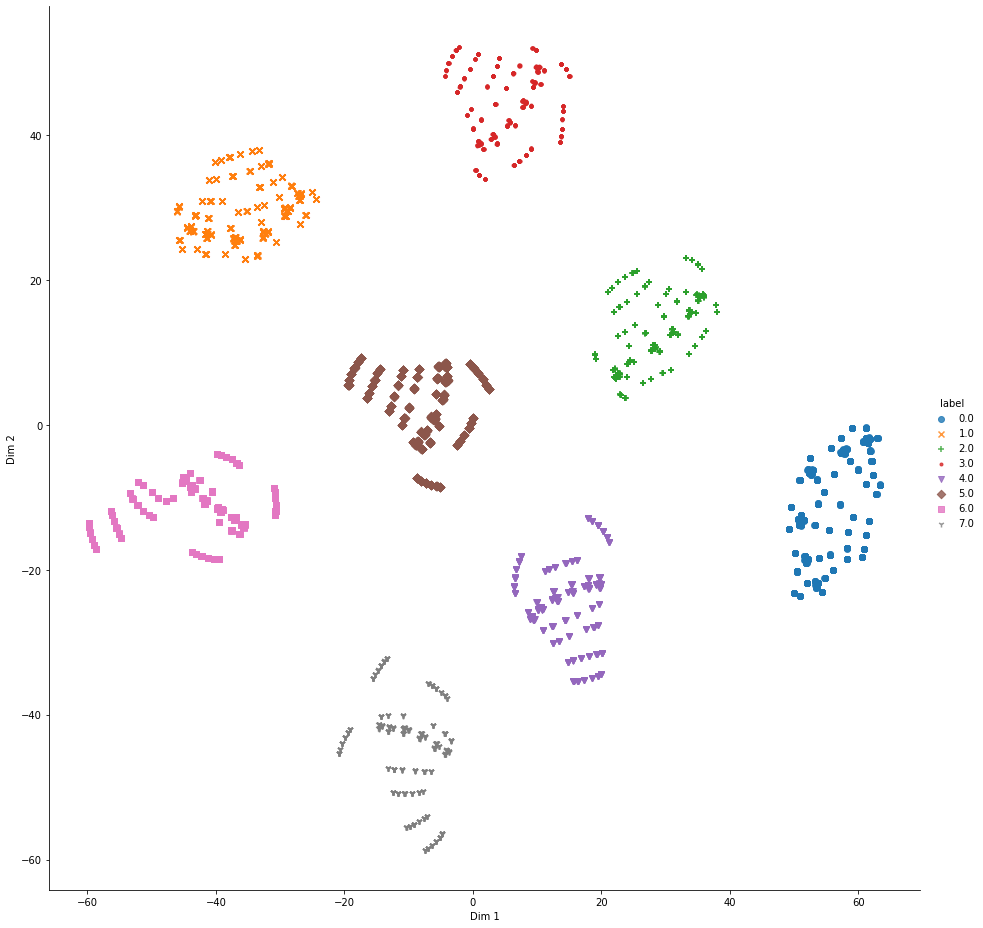
\includegraphics[width=150mm]{3/Fotos/Load_DACOMAT_t-sne.png}
%         \captionsetup{justification=centering,margin=1.25cm}
%         \caption{Representación de los vectores de deformaciones tras reducir la dimensión de 400 a 2}
%         \label{def_h}
%     \end{figure}  
    
%     \begin{figure}[H]
%         \centering
%         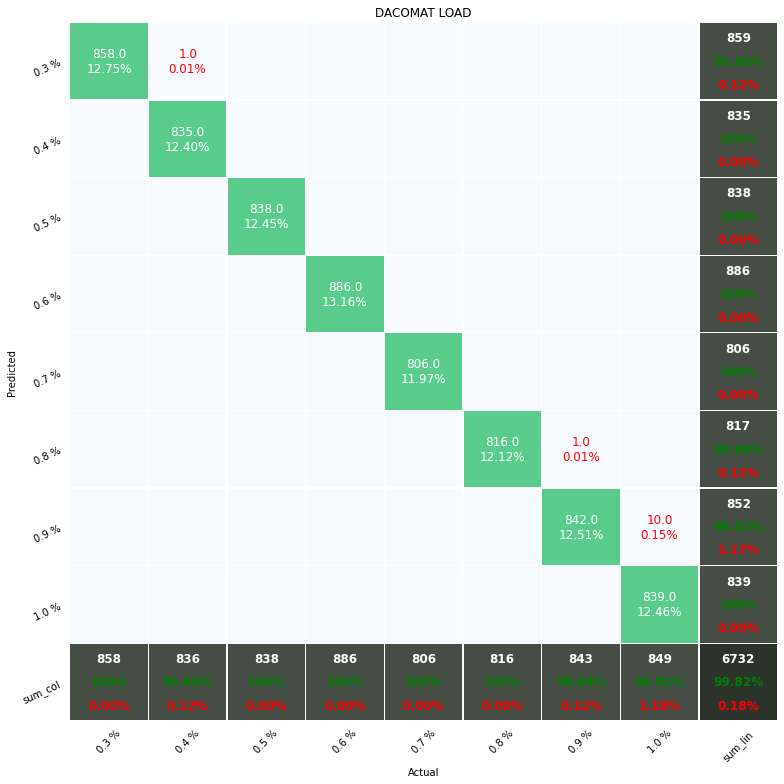
\includegraphics[width=150mm]{3/Fotos/Load_DACOMAT_confusion.png}
%         \captionsetup{justification=centering,margin=1.25cm}
%         \caption{Matriz de confusión}
%         \label{def_h}
%     \end{figure}  
    
%     \item[$\bullet$] \textbf{CLASIFICACIÓN DE TEMPERATURA}
    
%     \begin{figure}[H]
%         \centering
%         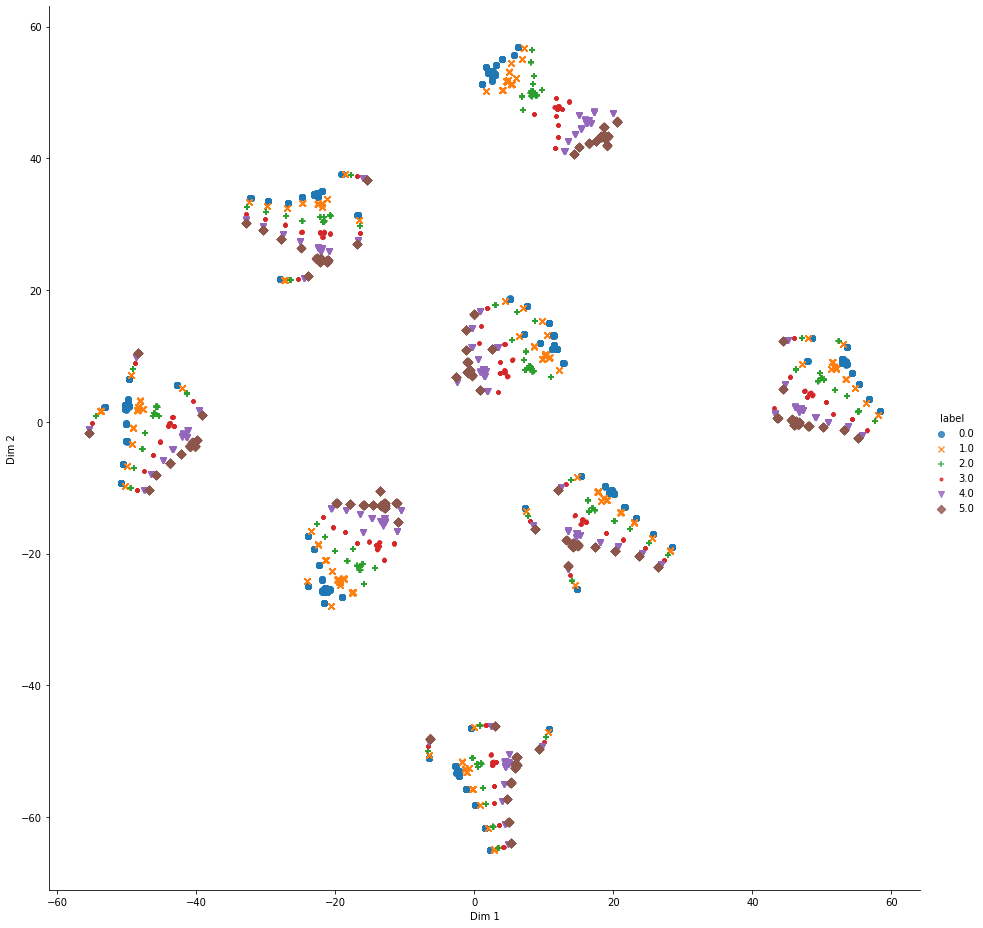
\includegraphics[width=150mm]{3/Fotos/Temperature_DACOMAT_t-sne.png}
%         \captionsetup{justification=centering,margin=1.25cm}
%         \caption{Representación de los vectores de deformaciones tras reducir la dimensión de 400 a 2}
%         \label{def_h}
%     \end{figure}  
    
%     \begin{figure}[H]
%         \centering
%         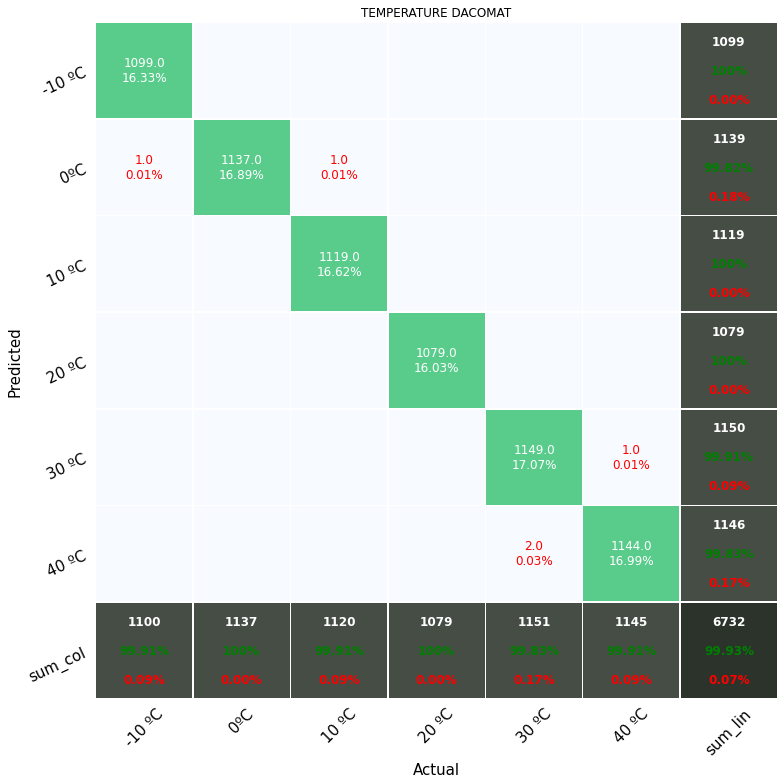
\includegraphics[width=150mm]{3/Fotos/Temperature_DACOMAT_confusion.png}
%         \captionsetup{justification=centering,margin=1.25cm}
%         \caption{Matriz de confusión}
%         \label{def_h}
%     \end{figure}  
    
%     \item[$\bullet$] \textbf{CLASIFICACIÓN DE CASO DE DAÑO}
    
%     \begin{figure}[H]
%         \centering
%         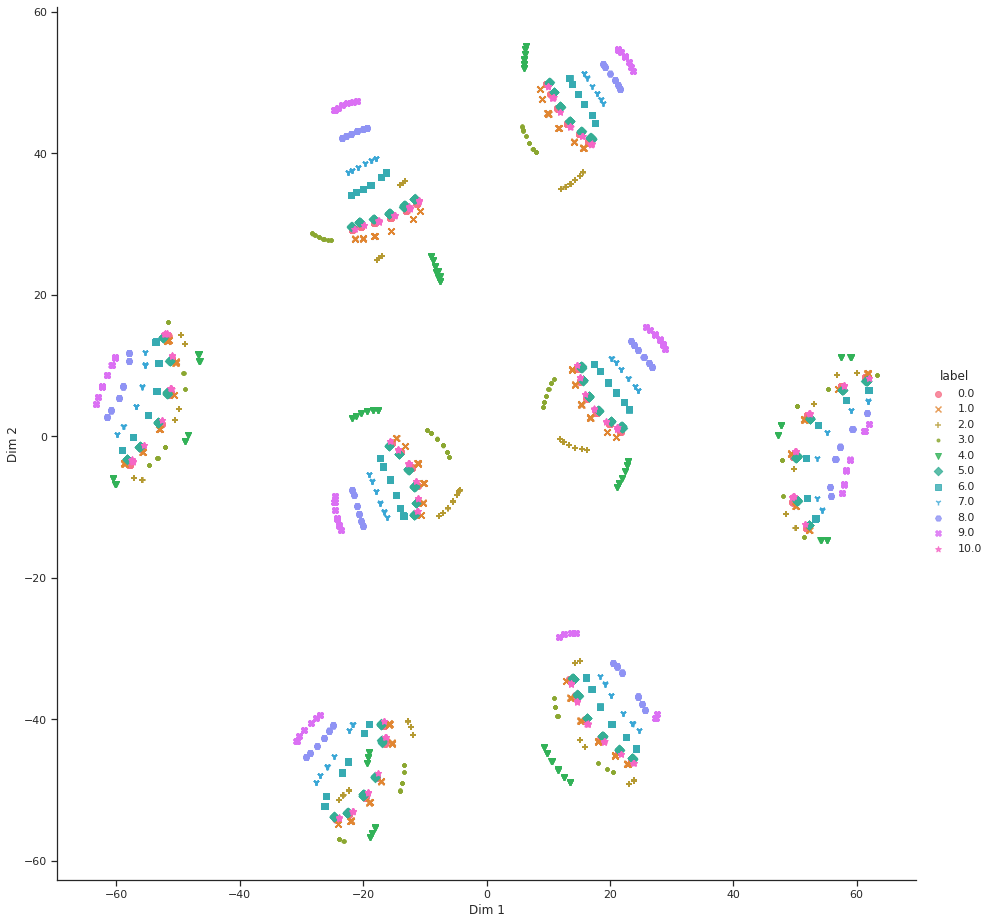
\includegraphics[width=150mm]{3/Fotos/Ty_Si_DACOMAT_t-sne.png}
%         \captionsetup{justification=centering,margin=1.25cm}
%         \caption{Representación de los vectores de deformaciones tras reducir la dimensión de 400 a 2}
%         \label{def_h}
%     \end{figure}  
    
%     \begin{figure}[H]
%         \centering
%         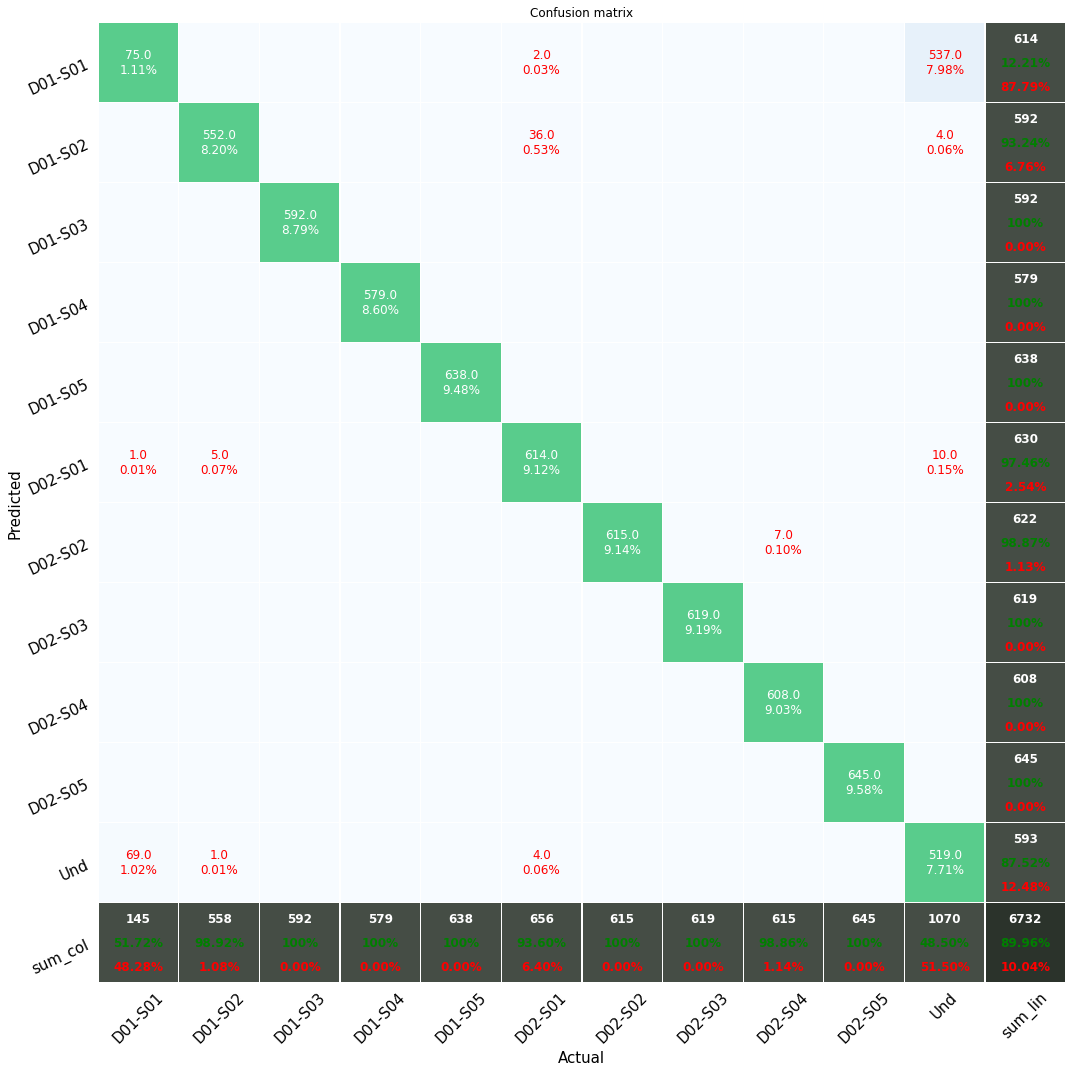
\includegraphics[width=150mm]{3/Fotos/Ty_Si_DACOMAT_confusion.png}
%         \captionsetup{justification=centering,margin=1.25cm}
%         \caption{Matriz de confusión}
%         \label{def_h}
%     \end{figure} 
    
% \end{itemize}
 
